\documentclass{article}
\usepackage[utf8]{inputenc}
\usepackage{graphicx}
\graphicspath{ {images/} }
\usepackage{wrapfig}
\usepackage[a4paper]{geometry}
%\userpackage[top=1 in, bottom=1.25 in, left=1.1 in, rigth=1.1 in] {geometry}
%\usepackage[paperwidth=17cm, paperheight=22.5cm, bottom=2.5cm, right=2.5cm]{geometry}
\title{ 
\LARGE \textsc{\textbf{Universidad De Sonora}} \\ \bigskip
\Large\textbf{ División de Ciencias Exactas y Naturales} \\
\textbf{Licenciatura En Física} \\ \bigskip
\bigskip
\textbf{Física Computacional I} \\ \bigskip

\Large \textbf{{Actividad 1}} \\ \bigskip
\textit{\textbf{"Climatología de la estación climática 26107"}}}
\\
\author{
\Large\textbf{ Gabriel Alberto López Monge} \\ \bigskip
\\ \bigskip
\Large\textbf{ Profr. Carlos Lizárraga Celaya}}
\\
\date{Enero 2021}
\begin{document}
\maketitle

\newpage
\section{\LARGE Introducción}
\begin{wrapfigure}{r}{0.25\textwidth} 
\caption{Océano y desierto 
\\ Guaymas, Sonora }
    \centering
    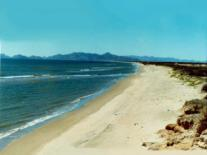
\includegraphics[width=0.25\textwidth]{1.jpg}
\end{wrapfigure}
 \large\textbf{La climatología es un tema muy grande para explorar debido a la amplía variación dependiendo de las región que se explore.
 \\ En este documento indagaremos acerca del clima de Guaymas-Vicam, Sonora una región ubicada a 140 kilómetros sureste de la capital.
 \\ A su ves es un lugar muy interesante para ver, debido a que es uno de los puntos donde se una el océano con el desierto, la variación de clima que se puede encontrar en este lugar es muy diverso e interesante.}
 
 \section{\LARGE Información}
 
\begin{figure}[h]
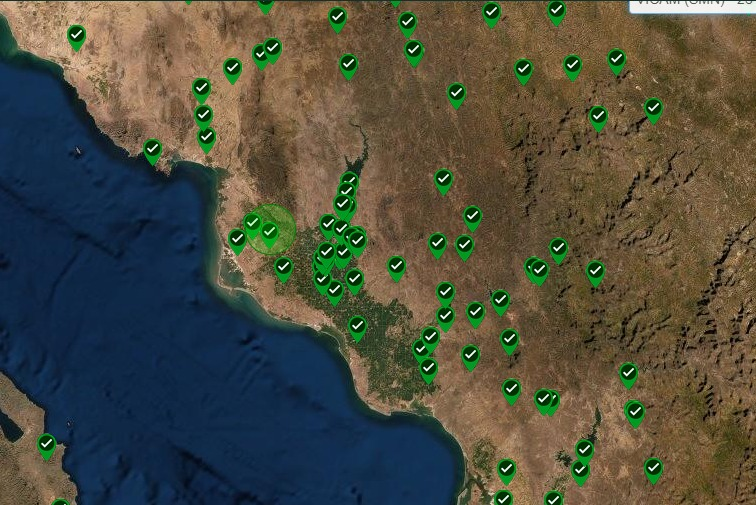
\includegraphics[width=8cm]{2.jpg} 
\\ \large\textbf{La estación se encuentra en el circulo verde}
\end{figure}


ESTACIÓN  : 26107\\
NOMBRE    : VICAM (SMN)\\
ESTADO    : SONORA\\
MUNICIPIO : GUAYMAS\\
SITUACIÓN : OPERANDO\\
ORGANISMO : CONAGUA-SMN\\
CVE-OMM   : Nulo\\
LATITUD   : 027.584°\\
LONGITUD  : -110.324°\\
ALTITUD   : 13 msnm

\section{\LARGE Estadística}
\begin{figure1}
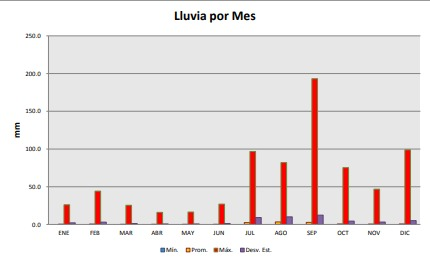
\includegraphics[width=15cm]{3.jpg} 
\end{figure1}
\newpage
\begin{figure1}
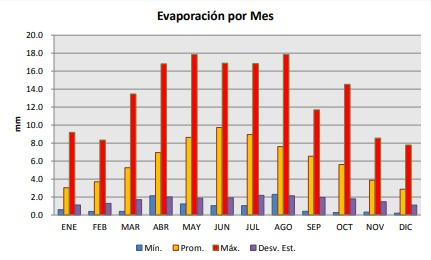
\includegraphics[width=15cm]{4.jpg} 
\end{figure1}
\newpage
\begin{figure1}
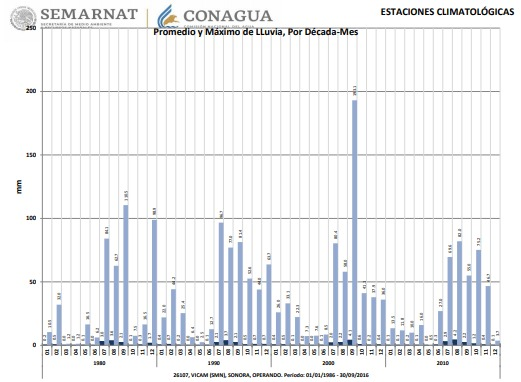
\includegraphics[width=15cm]{5.jpg} 
\end{figure1}
\newpage
\begin{figure1}
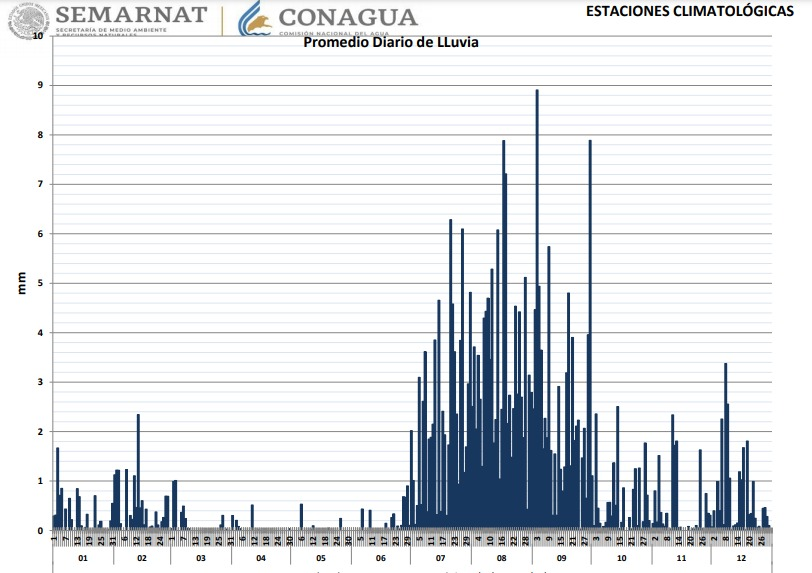
\includegraphics[width=15cm]{6.jpg} 
\end{figure1}
\newpage
\begin{figure1}
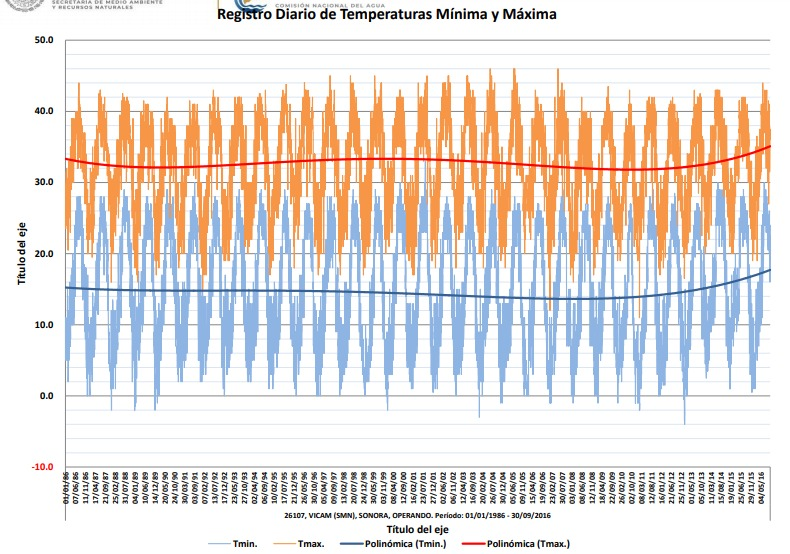
\includegraphics[width=15cm]{7.jpg} 
\end{figure1}
\newpage
\section{\LARGE Análisis}
\large\textbf{Como podemos observar en las gráficas anteriores, estas estadísticas obtenidas son similares en toda la región. 
\\Las lluvias son potenciadas en Septiembre, con poca precipitación entre abril y marzo.
\\
\\La evaporación se ve un alto indicie debido al tipo de bioma en el que nos encontramos.
\\
\\En promedio por década-mes la lluvia toda una variación, manteniendo el máximo en septiembre, en algunas décadas la lluvia inicia en el séptimo mes y se calma hasta el noveno.
\\
\\Sobre el promedio diarios de lluvias podemos observar que los picos de lluvias son en los meses de julio, agosto y septiembre. Las lluvias son muy altas a diferencia de mayo, abril y marzo. De igual manera los picos más altos de todo el año suelen ser a inicios del noveno mes.
\\
\\Las temperaturas son bástate radicales pero entendibles al saber que estamos hablando de una región árida como lo es Vicam, no tenemos temperaturas extremas, máximas de aproximadamente 43° y mínimos que no sobrepasan los -5° grados celcius.}

\section{\LARGE Apéndice}
¿Qué te pareció? Es una actividad muy intuitiva a la vez que, en mi caso, muy emocionante de realizar debido a que me gusta bastante la programación, tuve que ir aprendiendo a prueba y error cada comando a utilizar.
\\
\\
¿Cómo estuvo el reto? Me pareció bastante entretenida debido a que era mi primera vez utilizando este lenguaje, tuve que buscar mucho y memorizar bien los comandos.
\\
\\
¿Qué se te dificultó más? Se me dificulto el darle formato, aún es algo que no tengo dominado, es algo en lo que me estoy iniciando así que espero poderlo hacerlo mejor en un futuro, tal vez utilice comandos erróneos se ven mal pero el documento es legible.
\\
\\
¿Qué te aburrió? El utilizar overleaft es muy divertido, lo que no me termino de convencer fue el utilizar herramientas diferentes, como es Github.
\\
\\
¿Qué recomendarías para mejorar la primera Actividad? Utilizar algún tutorial básico debido a que me tomo bastante tiempo el volver a ver las clases debido a que no recordaba todos los comandos y el como utilizar las demás herramientas
\\
\\
¿Que grado de complejidad le asignarías a esta Actividad? Bajo para overleaf y alto para github, tuve muchos problemas para subir archivos.












\end{document}
